\begin{center}
 \textsc{Физбой, 10 класс. Финал.}
\end{center}
\vspace{0.01cm}
\hrule
\parindent=0mm

\task{ Над тонкостенным металлическим шаром, радиус которого $R = 5
  \mbox{ см}$, на высоте $h = 10 \mbox{ см}$ находится капельница с
  заряженной жидкостью. Капли жидкости падают из капельницы в
  небольшое отверстие в шаре. Определить максимальный заряд $Q_0$,
  который накопится на шаре, если заряд каждой капли $q = 1.8 \cdot 10^{-11}
  \mbox{ Кл}$. Радиус капель $r = 1 \mbox{ мм}$.}

\task{ Имеется батарейка с ЭДС $\eps_1$ и внутренним сопротивлением
  $r_1$, а также некоторое количество одинаковых батареек с ЭДС
  $\eps_2$. Если последовательно с батареей $\eps_1$ подключить
  некоторое количество батареек $\eps_2$ и нагрузку, то сила тока в
  цепи при любом количестве батареек $\eps_2$ будет одинаковой. Если
  же к батарейке $\eps_1$ параллельно подсоединить любое число
  батареек $\eps_2$ и ту же нагрузку, то сила тока через нее останется
  равной прежнему значению. Полярности всех батарей считать
  одинаковыми. Найдите сопротивление нагрузки $R$, а также внутреннее
  сопротивление $r_2$ батареек $\eps_2$.}

\task{ На некоторой планете может быть реализован следующий
  эксперимент. При плоских колебаниях математического маятника длиной
  $L = 3 \mbox{ м}$ максимальная сила натяжения нити отличается от
  минимальной в $k = 4$ раза, если максимальный угол отклонения равен
  значению угла $\alpha$. Такой же угол $\alpha$ с вертикалью образует
  нить маятника, если она вращается с периодом $T = 4 \mbox{ с}$ вокруг
  вертикальной оси, проходящей через точку подвеса. Определите
  ускорение свободного падения на данной палате.  \\
  \textit{Примечание.} Частота колебаний математического маятника
    зависит только от длины подвеса и ускорения свободного падения:
  $\omega = \sqrt{ g/L }$.  }

\task{ Большое число одинаковых плоских монет уложили плоскими
  сторонами вплотную друг к другу, разделив их круглыми кусочками
  бумаги, совпадающими по диаметру с монетами. Получившийся длинный
  цилиндр завернули бумагой в два слоя. Один из торцов этого цилиндра
  касается термостата, имеющего постоянную температуру $Т_1$. Ближайшую к
  термостату монету и сам термостат отделяет кусочек бумаги толщиной
  $h$. Сам цилиндр находится в воздухе, температура которого
  $Т_0$. Теплопроводность монет намного больше, чем теплопроводность
  бумаги. Диаметр монеты $d$, толщина монеты $Н$. Толщина слоя бумаги $h$
  ($h \ll d$). Теплопроводность материала бумаги --- $k$. Со временем
  установилось стационарное распределение температуры. Какое
  количество тепла получает цилиндр из монет от термостата в единицу
  времени?
\\
\textit{  Указание.} Тепловой поток $P$ сквозь тонкий слой вещества, площадь
  которого $S$, а толщина $dx$, равный количеству теплоты, проходящему
  сквозь этот слой в единицу времени, прямо пропорционален разности
  значений температуры его поверхностей $dT$ и обратно пропорционален
  его толщине:
  $P = -k S(dT/dx)$, где $k$ - коэффициент теплопроводности вещества.
}

\taskpic{ Один конец тонкой гибкой веревки с линейной плотностью $\rho$ тянут
  с постоянной горизонтальной скоростью на высоте $Н$ над шероховатой
  поверхностью. Второй конец веревки свободен. Длина части веревки,
  соприкасающейся с поверхностью равна $l_1$. Найдите длину веревки $l_2$,
  не касающейся поверхности. Коэффициент трения скольжения веревки по
  поверхности равен $k$.}{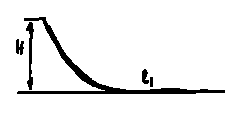
\includegraphics[width=4cm]{fb10_f_5.pdf}}

\task{ Для того, чтобы дорожные знаки были хорошо видны ночью, в
  серебряную краску, которой они покрываются, добавляют стеклянные
  шарики. Каким должен быть коэффициент преломления стекла, чтобы
  такой знак был светоотражающим?}
\setcounter{notask}{1}
